\documentclass[10pt,a4paper,twocolumn,twoside]{article}
\usepackage[utf8]{inputenc}
\usepackage[catalan]{babel}
\usepackage{multicol}
\usepackage{graphicx}
\usepackage{fancyhdr}
\usepackage{times}
\usepackage{titlesec}
\usepackage{multirow}
\usepackage{lettrine}
\usepackage[top=2cm, bottom=1.5cm, left=2cm, right=2cm]{geometry}
\usepackage[figurename=Fig.,tablename=TAULA]{caption}
\usepackage{hyperref}
\usepackage[ampersand]{easylist}
\usepackage{listings}

\lstset{
  breaklines=true,
  tabsize=2,
}

\captionsetup[table]{textfont=sc}

\titlespacing*{\section}{0pt}{0.5cm}{0.2cm}
\titlespacing*{\subsection}{0pt}{0.5cm}{0.2cm}


\graphicspath{{img/}}

\author{\normalsize\sffamily Kevin Martín Fernández}
\title{\huge{\sffamily Entorn de simulació per la captura d'imatges des de dron}}
\date{}

\newcommand\blfootnote[1]{%
  \begingroup
  \renewcommand\thefootnote{}\footnote{#1}%
  \addtocounter{footnote}{-1}%
  \endgroup
}

%No ident
\setlength\parindent{0pt}

%
%\large\bfseries\sffamily
\titleformat{\section}
{\large\sffamily\scshape\bfseries}
{\textbf{\thesection}}{1em}{}

\begin{document}

\fancyhead[LO]{\scriptsize Kevin Martín: Entorn de simulació per la captura d'imatges des de dron}
\fancyhead[RO]{\thepage}
\fancyhead[LE]{\thepage}
\fancyhead[RE]{\scriptsize EE/UAB TFG INFORMÀTICA: Entorn de simulació per la captura d'imatges des de dron}

\fancyfoot[CO,CE]{}

\fancypagestyle{primerapagina}
{
   \fancyhf{}
   \fancyhead[L]{\scriptsize TFG EN ENGINYERIA INFORMÀTICA, ESCOLA D'ENGINYERIA (EE), UNIVERSITAT AUTÒNOMA DE BARCELONA (UAB)}
   \fancyfoot[C]{\scriptsize ``Mes'' de 2019, Escola d'Enginyeria (UAB)}
}

%\lhead{\thepage}
%\chead{}
%\rhead{\tiny EE/UAB TFG INFORMÀTICA: TÍTOL (ABREUJAT SI ÉS MOLT LLARG)}
%\lhead{ EE/UAB \thepage}
%\lfoot{}
%\cfoot{\tiny{February 2015, Escola d'Enginyeria (UAB)}}
%\rfoot{}
\renewcommand{\headrulewidth}{0pt}
\renewcommand{\footrulewidth}{0pt}
\pagestyle{fancy}

%\thispagestyle{myheadings}
\twocolumn[\begin{@twocolumnfalse}

{
\vspace*{-1cm}
\maketitle
}

\thispagestyle{primerapagina}
%\twocolumn[\begin{@twocolumnfalse}
%\maketitle
%\begin{abstract}
\begin{center}
\parbox{0.915\textwidth}
{\sffamily\small
\textbf{Resum--} Resum
\\
\\
\textbf{Paraules clau-- }
Simulador, Drons, Terreny, Satelite, Multiespectre, Unreal Engine\\
\\
%\end{abstract}
}

\bigskip

{\vrule depth 0pt height 0.5pt width 4cm\hspace{7.5pt}%
\raisebox{-3.5pt}{\fontfamily{pzd}\fontencoding{U}\fontseries{m}\fontshape{n}\fontsize{11}{12}\selectfont\char70}%
\hspace{7.5pt}\vrule depth 0pt height 0.5pt width 4cm\relax}

\end{center}

\bigskip
%\end{abstract}
\end{@twocolumnfalse}]

\blfootnote{$\bullet$ E-mail de contacte: kevinmf94@gmail.com}
\blfootnote{$\bullet$ Menció realitzada: Enginyeria de Computació}
\blfootnote{$\bullet$ Treball tutoritzat per: Felipe Lumbreras Ruíz}
\blfootnote{$\bullet$ Curs 2018/19}

\vspace{-1cm}
\section{Introducció}
La simulació d'espais per a la generació d'imatges artificials és un àmbit en el qual es busca representa el món real de la forma més realista possible per tal de poder generar informació que en entorns reals ens representaria un perill o un cost econòmic elevat.
\\
\\
En aquest treball es vol aconseguir que mitjançant dades de mapes d'elevacions i imatges aèries de terrenys reals generar-ho en un entorn simulat per tal de poder generar imatges fictícies amb la màxima realitat possible per tal de generar datasets d'imatges per la utilització en diversos camps de l'aprenentatge computacional.

\section{Objectius}

En aquest apartat determinarem els diferents objectius del projecte en format de jerarquia per tal de veure la dependència entre els diferents objectius:

\begin{easylist}
\ListProperties(Progressive*=0.5cm)
& Analitzar
&& Investigar l'estat de l'art
&&& Estudiar AirSim
&&& Estudiar Carla SIMULATOR
&&& Estudiar proposta pròpia
&& Definir els objectius
&& Investigar motors gràfics
&&& Investigar Unreal Engine
&&& Investigar altres motors gràfics
&& Investigar els mapes d'altura
&& Investigar les imatges tant RGB com multiespectrals
&& Investigar webservices WMS
&& Investigar llibreries RPC
& Definir
&& Definir mòduls interessants pel projecte
&& Definir l'estructura del software
&& Definir plataformes utilitzades
&&& Definir els mòduls a desenvolupar
&&& Definir la comunicació entre els mòduls
&&& Definir estructura de les dades que rebrà Unreal Engine
& Desenvolupar
&& Desenvolupar mòdul de transformació i obtenció de dades
&&& Desenvolupar el mòdul de transformació de dades d'altura i textures
&&& Desenvolupar l'importador de dades en Unreal Engine
&& Desenvolupar mòdul gràfic (Ureal Engine)
&&& Desenvolupar la interfície del menú
&&& Desenvolupar el mòdul per importar fitxers personalitzats en Unreal Engine
&&& Desenvolupar codi per la generació del terreny
&&& Desenvolupar codi per la generació dels materials
&&&& Visualitzar diferents materials (RGB, Multi-espectre, ...)
&&& Desenvolupar codi de servidor per control del vehicle
&& Desenvolupar mòdul de scripting
&&& Desenvolupament client que controlarà el vehicle
&& Integrar els mòduls de AirSim en Unreal Engine
&&& Integrar mòdul de Drons en el projecte
&&& Integrar mòdul de Segmentació en el projecte
&& Desenvolupar altres capes d'informació
& Testejar
&& Fer provàs del mòdul de transformació de dades
&&& Provar amb dades locals
&&& Provar amb dades externes
&& Fer provàs del mòdul gràfic
&& Fer provàs del mòdul de control per scripting
&&& Elaborar script d'exemple
&&& Provar script d'exemple
& Documentar
&& Redactar informe inicial
&& Redactar informe de seguiment I
&& Redactar informe de seguiment II
&& Redactar l'informe final
&& Elaborar proposta de presentació
&& Elaborar pòster
&& Gestionar la documentació del dossier
\end{easylist}

\newpage
\section{Metodologia}

En aquest projecte s'ha decidit utilitzar una metodologia de tipus Agile\cite{agile}, ja que això ens permetrà identificar d'una forma millor les petites parts de les quals es compon aquest projecte, a més a més d'adaptar-se als canvis imprevistos. En concret s'ha escollit la tècnica Kanban\cite{kanban} que consisteix en organitza el nostre backlog (tasques de curta duració) en
targetes que ficarem en un taulell segons en quin punt del cicle de vida de la tasca es trobi (pendent, començada, ...) per això s'ha decidit utilitzar l'eina Trello\cite{trello} que permet de forma visual crear targetes i moure-les entre les diferents llistes.

\subsection{Diagrama de Gant}

Per tal de gestionar el projecte també s'ha empleat un diagrama de Gant elaborat amb excel. En aquest diagrama contemplarem les diverses tasques i subtasques per tal de fer una previsió del treball a realitzar, el temps aproximat que trigarem per cada tasca, això ens permetrà fer una aproximació del temps que ens comportarà el projecte d'aquesta forma podrem determinar la viabilitat.

\section{Estat de l'art}
\label{estatart}

Actualment existeixen diverses aplicacions per la generació d'imatges en entorns que simulen la realitat amb la finalitat de generar dades per algoritmes d'aprenentatge.
En aquest àmbit unes de les més importants és AirSim\cite{airsim} desenvolupat per Microsoft i Carla SIMULATOR\cite{carla} desenvolupat pel centre de visió per computador.

\subsection{AirSim}
AirSim és un simulador gràfic elaborat en Unreal Engine\cite{unreal} aquest simulador té la finalitat de generar imatges en un entorn totalment fictici, incorpora diversos mòduls que ens ofereix les següents funcionalitats (podem veure un exemple a la figura \ref{fig-airsim}):
\\
\begin{easylist}[itemize]
& Simulació de cotxes
& Simulació de drons
& Compatibilitat amb controladors reals de drons
& Gravació 
& Vista de mapa de profunditats
& Vista segmentada
& Efectes de pluja
& Control d'il·luminació segons l'hora diària
& Control dels vehicles mitjançant scripts en python
\end{easylist}

\begin{figure}[!h]
\centering
  	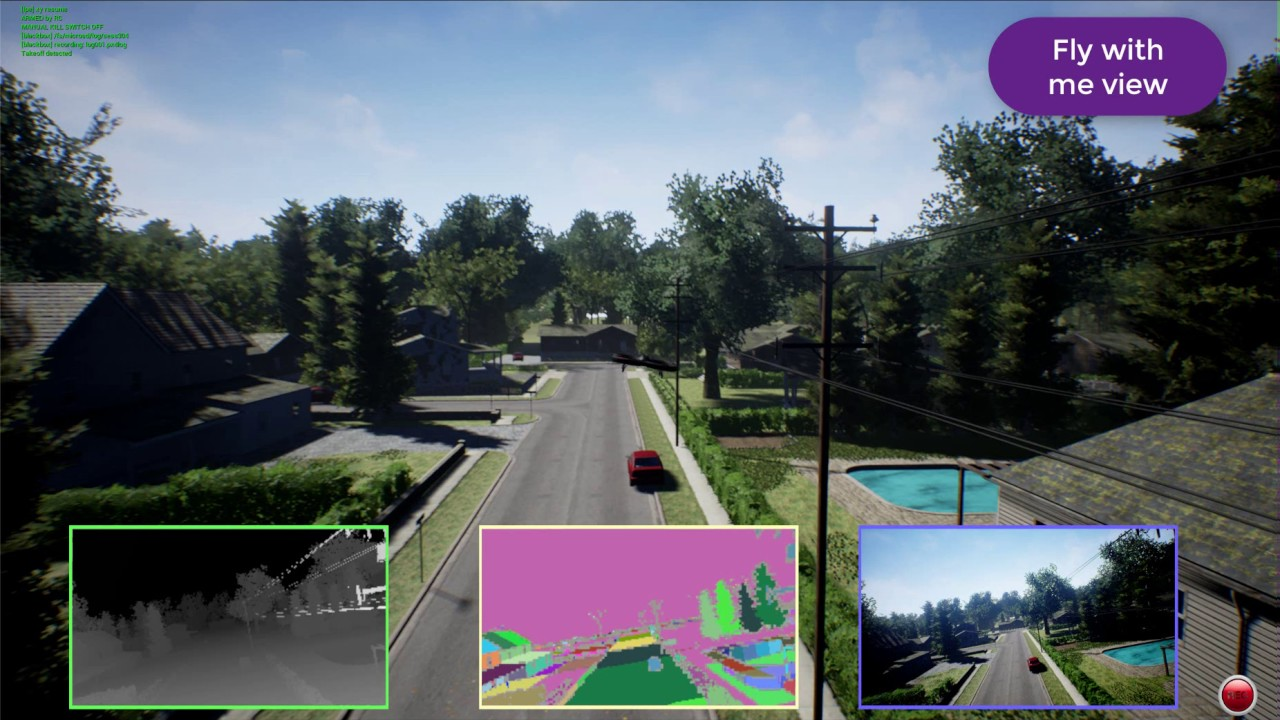
\includegraphics[width=0.4\textwidth]{airsim}
	\caption{Simulador Airsim}
	\label{fig-airsim}
\end{figure}

\newpage
\subsection{Carla SIMULATOR}
Carla és un simulador gràfic elaborat en Unreal Engine aquest simulador té la finalitat de generar imatges en entorn fictici amb la màxima realitat possible per generar imatges que serveixin per a l'aprenentatge de xarxes neuronals capaces de conduir un cotxe autònom de forma segura tenint en compte els casos poc probables que no es podrien generar en un entorn físic. Aquest entorn compte amb les següents funcionalitats:

\begin{easylist}[itemize]
& Simulació de cotxes
& Vista de mapa de profunditats
& Vista segmentada
& Simulació de tràfic
& Control dels actors amb scripts de python
\end{easylist}

\section{Estructura del projecte}

Per tal de determinar l'estructura del nostre projecte s'han estudiat vàries alternatives vistes a l'apartat \ref{estatart} en les quals es pot veure com estan organitzats altres projectes similars. En aquest apartat veurem l'estructura de diferents projectes amb l'objectiu de decidir l'estructura del projecte i diferents llibreries.

\subsection{AirSim} 

AirSim està compost per múltiples mòduls escrits en diversos llenguatges com es pot veure a continuació:
\\
\begin{easylist}[itemize]
& \textbf{AirLib (C++)}: Mòdul per a Unreal Engine que proporciona les classes bàsiques per comunicar-se mitjançant el protocol RCP i control dels vehicles simulats.
& \textbf{DroneServer (C++)}: Servidor per rebre ordres de Dron mitjançant RCP.
& \textbf{DroneShell (C++)}: Client de consola per enviar ordres al mòdul de dron.
& \textbf{PythonClient (Python)}: Client que envia ordres mitjançant RCP, també incorpora codi per al tractament, segmentació d'imatges, etc.
& \textbf{SGM (C++)}: Codi per tractar imatges i generar les vistes segmentada i stereo.
& \textbf{Unity (C\# i C++)}: Demostració en el motor gràfic Unity, incorpora una sèrie de mòduls per Unity per visualitzar la informació d'AirSim.
& \textbf{Unreal Engine (C++)}: Demostració en el motor gràfic Unreal Engine, incorpora una sèrie de mòduls per Unreal Engine per visualitzar la informació d'AirSim.
\end{easylist}

\subsection{Carla SIMULATOR}

Carla SIMULATOR està compost per múltiples mòduls com podem veure en la figura \ref{fig-carlamodules} escrits en diversos llenguatges com es pot veure a continuació:

\begin{figure}[!h]
\centering
  	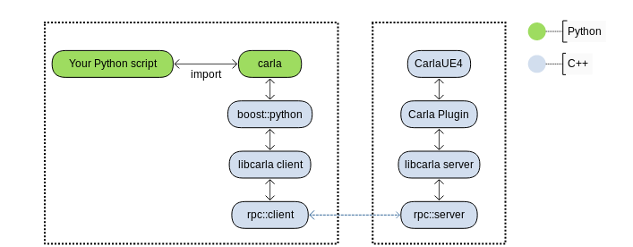
\includegraphics[width=0.5\textwidth]{carlamodules}
	\caption{Relació entre els mòduls de Carla}
	\label{fig-carlamodules}
\end{figure}

\begin{easylist}[itemize]
& \textbf{LibCarla (C++)}: Llibreria principal de Carla
& \textbf{Unreal (C++)}: Motor gràfic amb el plugin de carla, que incorpora totes les funcionalitats afegides a Unreal.
& \textbf{PythonAPI (Python)}: API que ens permetrà enviar comandes al mòdul de Carla que fa de servidor, aquest api serveix per crear scripts propis.
\end{easylist}

\subsection{Estructura escollida}

Analitzant diversos projectes de característiques similars s'ha decidit per una estructura pròpia com podrem veure en la figura \ref{fig-dronsimulatormodules} podent reutilitzar alguns dels petits mòduls open-source d'altres projectes. S'ha pres aquesta decisió a causa del fet que els altres projectes es basen en la creació terrenys predefinits mitjançant l'entorn d'Unreal, contrari a la finalitat d'aquest projecte en el qual es volen elaborar de forma automàtica terrenys a partir de dades reals.

\begin{figure}[!h]
\centering
  	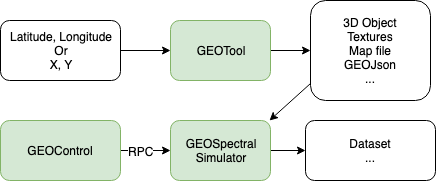
\includegraphics[width=0.45\textwidth]{structuretfg}
	\caption{Estructura DronSimulator}
	\label{fig-dronsimulatormodules}
\end{figure}

En el nostre projecte constarà d'aquests mòduls:
\\
\begin{easylist}[itemize]
& \textbf{GEOTool (Python)}: Aquest mòdul té la finalitat de donar les eines necessàries per a l'obtenció i adaptació de les dades proveïdes per webservices estàndard en l'àmbit de l'obtenció de dades geogràfiques amb l'objectiu de poder importar-les en qualsevol motor gràfic, podent generar diferents capes d'informació per als terrenys descarregats.
& \textbf{ScriptAPI (Python)}: API que ens permetrà fer scripts en Python per tal de controlar la càmera en l'entorn gràfic. D'aquesta forma també ens permetrà l'obtenció d'imatges en l'entorn Unreal Engine.
& \textbf{Unreal Engine Simulator (C++)}: Incorporarà tot el motor gràfic i connectors necessaris per a la comunicació amb els fitxers generats amb el mòdul GEOTool, visualització de dades, obtenció d'imatge, etc.
\end{easylist}

\section{Mòdul GeoTools}

Mòdul generat en Python amb l'objectiu d'obtenir informació de mapes d'elevacions, ortofotos, etc. Amb l'objectiu posterior de fer un tractament d'aquestes dades per la generació de terrenys tridimensional i informació en format visible per tal de poder visualitzar-ho en un motor gràfic de tipus Unreal, Unity, OpenGL, etc.

\subsection{Obtenció de dades}

Amb l'objectiu d'obtenir dades geogràfiques s'ha optat per la comunicació amb els estàndards proposats per l'Open Geospatial Consortium\cite{ogc}: Web Map Service\cite{wms} encarregat de posar a disponibilitat dades d'imatge com poden ser ortofotos d'una zona geogràfica seleccionada i Web Coverage Service\cite{wcs} encarregat de retornar informació referent a les elevacions de terreny en una zona geogràfica concreta. Per tal d'obtenir dades es fan peticions HTTP a les direccions web oferides per distintes institucions que segueixen els estàndard anomenats, en aquest cas s'ha realitzat proves amb l'Institut Cartogràfic i Geològic de Catalunya\cite{icgc}.

\subsubsection{Fitxer de configuració}

Per tal de determinar quines dades volem obtenir i de quins webservices l'aplicació accepta per paràmetre un fitxer de configuració en format JSON que ens permet determinar diferents propietats de les dades que demanarem com es pot veure en l'apèndix \ref{appendix:geotoolconfig}. En aquest fitxer es pot configurar els següents paràmetres:

\begin{easylist}
& \textbf{Type}: Fa referència al tipus de coordenades que li passarem, pot ser latlong o xy en el primer cas farà la corresponent transformació al format UTM (xy)
& \textbf{Coordinates}: Coordenades sobre les quals volem fer la petició en el format indicat en el camp type. Si s'escull "xy" es definirà els atributs x, y en cas d'escollir "latlong" definirem els atributs lat, long.
& \textbf{Dimensions}: En aquesta secció escollirem les dimensions que volem que es demanin en les peticions per tal de mantenir la mateixa zona geogràfica.
&& Bbox: Aquestes seran les dimensions de la zona que volem obtenir amb les que es calcularà els límits que delimitaran la zona.
&& Texture: Aquesta serà la resolució que obtindrem per les diferents textures.
& \textbf{Wcsurl}: URL al webservice que ens donarà les dades d'altures.
& \textbf{Outputwcs}: Nom de sortida del fitxer generat per les altures
& \textbf{Formatwcs}: Format del fitxer generat per les altures. Disponibles: raw, obj (Objecte 3D)
& \textbf{Wmsrequests}: Array amb cada una de les peticions que farem a diferents WMS per tal d'obtenir vàries imatges
&& Url: URL al webservice WMS
&& Layers: capa o capes que volem obtenir d'aquests webservice
&& Output: Nom del fitxer de sortida
&& OutputFormat: Format del fitxer de sortida. Disponibles: JPG
\end{easylist}

\subsection{Estructura de GEOTool}

\subsection{Generació de Terrenys a partir dun mapa d'altures}
En aquesta secció s'explicarà les diverses formes que s'han optat per generar terrenys que puguin ser interpretats en diferents motors gràfics.

\subsubsection{Format RAW}
El format RAW és un format pla que es basa en guarda en valors de 16 Bytes totes les altures en format binari tenim com a referència del mar el valor 128, i afegits en el fitxer un darrere de l'altre. Aquest format és acceptat per al creador de terrenys d'Unreal i Unity, però té certes limitacions de dimensions que s'han de complir especificades a l'editor en crear el terreny que fa que es perdi el control de la malla generada, les coordenades de textura no coincideixen amb la textura que es vol aplicar al terreny. Motius pels quals s'ha optat per afegir la generació de l'objecte 3D en format estàndard definit nosaltres l'objecte com es podrà veure en l'apartat \ref{mesh3d}, ja que aquestes limitacions fan que es facin vàries adaptacions no estàndards perquè es pugui visualitzar correctament.

\subsubsection{Generació de malla 3D}
\label{mesh3d}
Per tal d'importar terrenys en els motors gràfics s'ha optat per generar una malla 3D en format Wavefront obj\cite{wavefrontobj} format compatible amb qualsevol editor 3D, motor gràfic, etc. Aquest format dóna la llibertat per tal de controla la distància entre els vèrtexs, on s'aplicarà la textura i quines seran les normals dels vèrtexs fent que el terreny sigui suavitzat.
\\
\\
Com que el tractament amb bucles és lent s'ha realitzat tots els càlculs amb la llibreria NumPy aprofitant l'eficiència que incorpora aquesta llibreria amb el càlcul de matrius pel qual s'ha adaptat el problema com podem veure en el codi disponible en l'annex \ref{appendix:generateobj}.
\\
\\
Per la generació d'objectes cal definir 4 tipus d'objectes:

\begin{easylist}
& \textbf{Vèrtex}: Són cada un dels punts en el món, van definits pels índexs segons llegui'm la graella d'elevacions, es multipliquen per un K (Distancia entre els vèrtexs segons la distància que ens indiqui el mapa d'elevacions obtingut).

& \textbf{Vèrtex de textura}: Vèrtex amb dos components x, y compresos entre el 0 i 1 que indican la correspondència entre els punts d'una textura i la malla en la qual es vol aplicar aquella textura. Aquestes propietats es calcularien amb les equacions \ref{equation:u} i \ref{equation:v}.
\begin{equation}
\label{equation:u}
u = f(columna) = columna / (ample - 1)
\end{equation}
\begin{equation}
\label{equation:v}
v = f(fila) = 1 - (fila / (altura - 1))
\end{equation}

& \textbf{Normal del vèrtex}: Vectors que ens indica la direcció en la qual es reflecteix la llum per a cada vèrtex de l'objecte. Per tal de calcular aquestes normals cal el pas previ de calcular les normals de cada cara, aquestes no seran introduïdes al fitxer final, ja que aquestes les genera'n els motors per defecte segons l'ordre en el qual indiquem els vèrtexs de les cares com es veurà més endavant.

&& Generació de normals de cares: Per tal de generar les normals d'una cara un cop sapiguem la relació entre les cares se seguirà el patró vist en la figura \ref{fig-normalcara} on seguirem l'equació \ref{equation:u} per al càlcul de la normal de la cara. $\dot{\vec{A}}$ i, realitzarem el producte vectorial $\vec{C} = \vec{B}*\vec{A}$ i per
últim normalitzarem el vector $\vec{Normal} = \frac{\vec{C}}{\mid\vec{C}\mid}$.

&& Generació de normals en els vèrtexs: Per tal de generar el vector normal per a cada vèrtex utilitzarem l'estructura que es pot veure en la figura \ref{fig-normalvertex} aplicant la següent formula a cada vèrtex on V correspon als vèrtexs i F a les cares de la figura \ref{fig-normalvertex}:
\begin{equation}
\vec{NormalV} = \vec{F1} + \vec{F2} + \vec{F3} + \vec{F4} + \vec{F5} + \vec{F6}
\end{equation}
\begin{equation}
\vec{NormalV} = \frac{\vec{NormalV}}{\mid\vec{NormalV}\mid}
\end{equation}

& \textbf{Cares}: En aquest punt determinarem quina és la unió dels vèrtexs per tal de generar les diferents cares de la malla, en aquesta implementació s'ha decidit per fer triangulació, és a dir, per cada quadrat de la nostra malla generarem 2 cares triangulars. És important generar les cares mantenint l'ordre dels vèrtexs contrari a les agulles del rellotge, d'aquesta forma els motors gràfics determina'n que la normal de la cara apuntarà cap dalt visualitzant correctament la malla 3D.

\end{easylist}

\begin{figure}[!h]
\centering
  	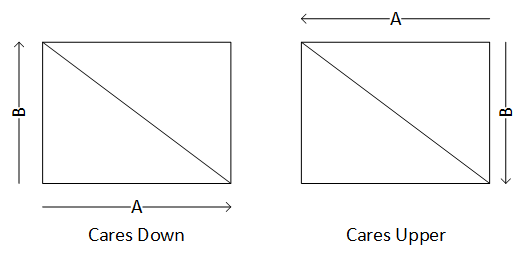
\includegraphics[width=0.4\textwidth]{caranormal}
	\caption{Patró per càlcul de normals en les cares}
	\label{fig-normalcara}
\end{figure}

\begin{figure}[!h]
\centering
  	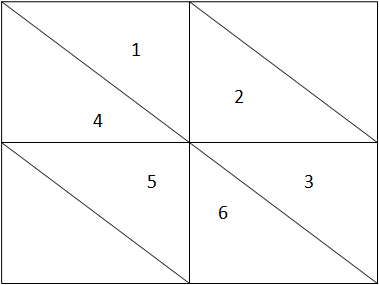
\includegraphics[width=0.2\textwidth]{vertexnormal}
	\caption{Patró per càlcul de normals en un vèrtex}
	\label{fig-normalvertex}
\end{figure}

\newpage
Un cop realitzat el procés de generació l'aplicació haurà generat una malla que podem obrir en qualsevol editor com podem veure en la figura \ref{fig-meshlab}

\begin{figure}[!h]
\centering
  	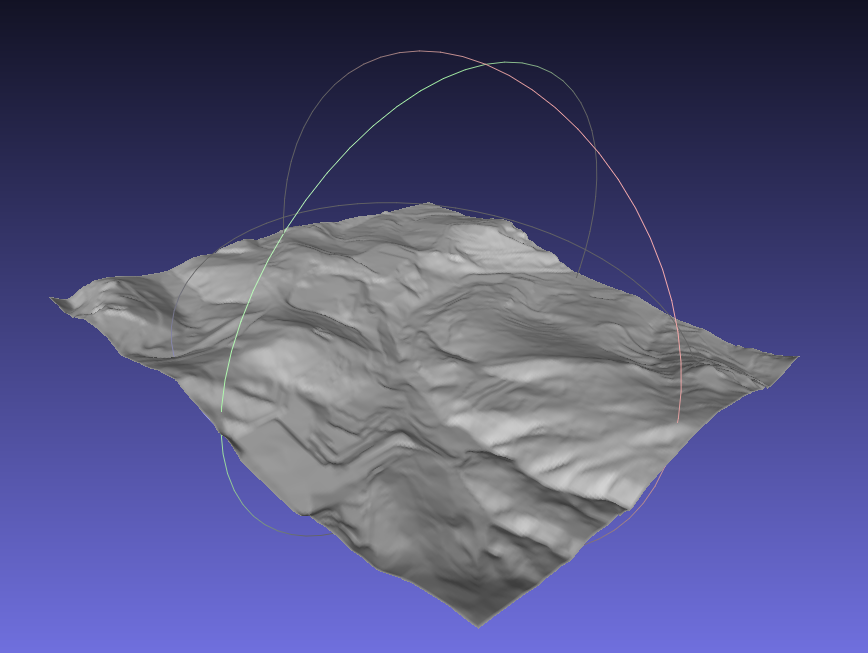
\includegraphics[width=0.35\textwidth]{mesh_example_meshlab}
	\caption{Malla d'un terreny visualitzada en l'aplicació MeshLab}
	\label{fig-meshlab}
\end{figure}

\section{Mòdul: Simulador}

En aquesta secció explicarem els diferents punts dels quals es compon el mòdul de simulació amb el que es cerca l'objectiu de posar a disposició una eina que ens permeti simular un viatge amb dron per sobre d'un terreny obtenint imatges des de diferents càmeres.

\section{Mòdul Scripting}

\section{Conclusions}


\section*{Agraïments}


\begin{thebibliography}{11}
\bibitem{agile}
Agile software development
\\ \url{https://en.wikipedia.org/wiki/Agile_software_development}
[19/02/2019]

\bibitem{kanban}
Kanban
\\ \url{https://www.iebschool.com/blog/metodologia-kanban-agile-scrum/} [19/02/2019]

\bibitem{trello}
Trello - \url{https://trello.com/} [19/02/2019]

\bibitem{airsim}
AirSim - \url{https://github.com/Microsoft/AirSim} [19/02/2019]

\bibitem{carla}
Carla SIMULATOR - \url{http://carla.org} [19/02/2019]

\bibitem{unreal}
Unreal Engine - \url{https://www.unrealengine.com/en-US/what-is-unreal-engine-4} [09/03/2019]

\bibitem{ogc}
Open Geospatial Consortium (OGC) -  \url{http://www.opengeospatial.org/} [08/04/2019]

\bibitem{wms}
Web Map Service (WMS) -  \url{https://www.opengeospatial.org/standards/wms} [08/04/2019]

\bibitem{wcs}
Web Coverage Service (WCS) -  \url{https://www.opengeospatial.org/standards/wcs} [08/04/2019]

\bibitem{icgc}
Institut Cartogràfic i Geològic de Catalunya (ICGC) - \url{http://www.icgc.cat/ca/} [08/04/2019]

\bibitem{wavefrontobj}
Wavefront .obj file - \url{https://en.wikipedia.org/wiki/Wavefront_.obj_file} [09/04/2019]


\end{thebibliography}

\newpage
\appendix

\section*{Apèndix}

\setcounter{section}{1}

\subsection{JSON d'exemple per la configuració de GEOTool}
\label{appendix:geotoolconfig}
\lstinputlisting{geotoolconfig.json}

\subsection{Codi per la generació d'una malla 3D a partir d'un fitxer d'altures}
\label{appendix:generateobj}
\lstinputlisting[language=Python]{generateobj.py}

\subsection{Secció d'Apèndix}



\end{document}

